% 来源：OEBPS/Text/Section0001_split_007.xhtml#sigil_toc_id_54

\BookChapter{41}
\section[第41章\q 麦嘉华：被称为末日博士的亿万富豪]{第41章\\ 麦嘉华：被称为末日博士的亿万富豪}

\begin{figure}[htbp]
\centering
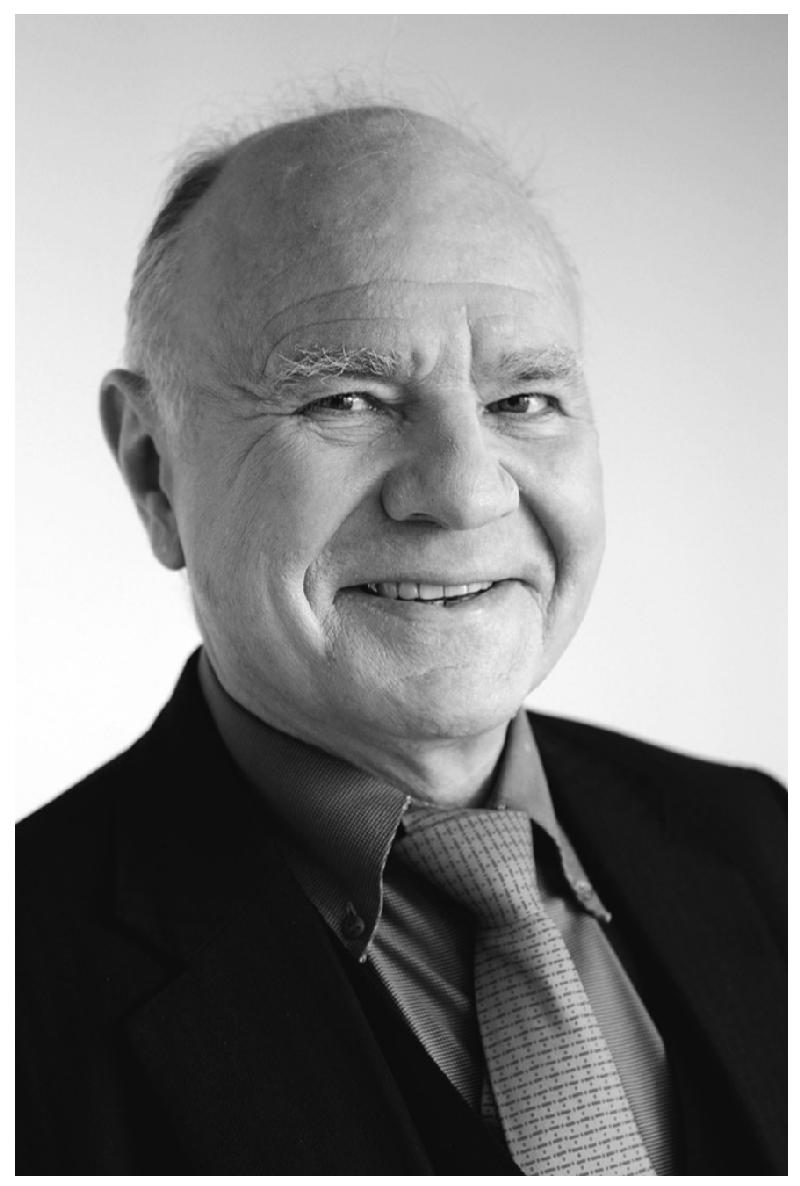
\includegraphics[width=0.40\linewidth,keepaspectratio]{image/麦嘉华肖像.jpg}
\caption*{麦嘉华}
\end{figure}

麦嘉华有限公司董事长，《股市荣枯及厄运报告》作者

麦嘉华做了一份投资通讯，叫作《股市荣枯及厄运报告》，他对市场的看法，这个名字应该会给你一个提示！但是这个来自瑞士的亿万富豪，可不是个一般人。我和麦嘉华认识好多年了，他这个人的生活多姿多彩，说话直来直去，在投资上总是喜欢唱反调，是个标准的逆向投资者，他总是遵循18世纪的投资大师巴伦·罗斯柴尔德的教诲：“最好的买入时机就是街上血流成河的时候。”就像约翰·邓普顿爵士，他追逐的股票，都是别人不重视或者远远避开的东西。这正是很多人聚焦美国股市的时候，只有麦嘉华转向亚洲市场寻找成长股投资机会的原因。麦嘉华经常直言不讳地批评所有国家的中央银行，特别是美联储，他谴责美联储把世界经济搞得很不稳定，因为美联储大搞量化宽松，把数以万亿的美元货币投到市场里，让市场好像发了洪水一样，而这些货币可以说都是凭空“印”出来的。

麦嘉华得到一个外号，叫作“末日博士”，这是因为他多年出版《股市荣枯及厄运报告》，持续不断地预测当前市场最流行的资产定价过高，末日即将来到，价格肯定暴跌。伦敦的《星期日泰晤士报》写道：“麦嘉华说的东西，没有人愿意听。”是的，但麦嘉华说的东西往往是对的，特别是1987年，他预测到了美国股市大崩盘，赚到了很大一笔钱。

麦嘉华的父亲是一名骨科医生，他的妈妈来自瑞典一个经营旅馆的家族。麦嘉华在苏黎世大学获得经济学博士，进入一家全球性投资企业怀特·维尔公司，从此开始金融投资生涯。1973年，麦嘉华转到亚洲，从此再也没有回去，一直都在亚洲工作生活。麦嘉华的公司设在中国香港，他住的度假别墅在泰国清迈，这让他像看演出坐在第一排一样，近距离看到了中国令人不可思议的经济大转变，从一个陷入泥沼的经济体，转变成驱动地区增长的引擎。现在，麦嘉华成为数一数二的亚洲市场研究专家。

麦嘉华的特立独行是出了名的，他非常开心地知道别人封他为“世界夜生活鉴赏家”，他也是世界各地金融论坛上很受欢迎的演讲人，经常作为嘉宾在各大电视新闻节目上发表评论。麦嘉华是投资界享有盛名的巴伦圆桌会议成员，按照独立观察人士的分析，他推荐的股票收益率是最高的，过去连续12年的平均年化收益率为23\%。麦嘉华写了几本关于亚洲市场的投资书籍，他是麦嘉华有限公司的董事长，这是一家设在中国香港的投资顾问和投资基金公司。麦嘉华说的英语带有浓浓的瑞典口音，他也从来不太把自己当回事儿，一点儿投资大腕儿的架子也没有。2014我在太阳谷举办经济论坛，麦嘉华应邀参加，我在台上现场采访了他，下面是访谈的内容节选。

\begin{BookQuote}
\textbf{罗宾斯：}你说过，现在世界上有三个最大的投资谎言，到处都在推销，请给我们详细讲讲。
\end{BookQuote}

\begin{BookQuote}
\textbf{麦嘉华：}我觉得，所有宣传推销的东西都是谎言！其实真理往往非常简单！不过，我的意思是，你看，我碰见过很多非常诚实的人，但是不幸的是，在你一生中，你会碰到很多像推销员一样的金融投资顾问，你本来觉得人都是非常诚实的，但是我必须诚实地告诉你：每个人都想推销给你你梦寐以求的投资。但是，按照我多年的经验，我担任过好多个投资基金公司的董事长，对这种事看得太多了，一般来说，客户只能赚到一点儿钱。但是这些基金经理——这些卖基金的投资理财顾问，他们走的时候都会带走一大笔钱。客户赚不到什么钱，钱都让这些基金经理和基金销售人员赚走了。
\end{BookQuote}

\begin{BookQuote}
\textbf{罗宾斯：}那么投资者应该转战哪里？
\end{BookQuote}

\begin{BookQuote}
\textbf{麦嘉华：}投资世界有各种各样不同的理论，基本上讲的都是有效市场理论。这些理论说，市场是有效的。换句话说，你投资的时候最好就是只买指数基金，个人选股基本上是没有用的。但是我可以告诉你，我知道有很多基金经理，长期来看确实明显跑赢了市场，领先幅度很明显。我相信有些人在分析公司上确实有一套，他们要么是很好的会计师，要么是确实很有本事。
\end{BookQuote}

\begin{BookQuote}
\textbf{罗宾斯：}你觉得近期市场怎么样？
\end{BookQuote}

\begin{BookQuote}
\textbf{麦嘉华：}我觉得在新兴市场国家还存在一些风险，现在要买这些新兴市场的货币和股票，时间还太早，但是要买美国的股票，时间就太晚了。标准普尔指数都到1800点之后，我就不再想买美股了。我看不到美股有任何投资价值。所以说，最好就是去喝酒、跳舞，尽情享乐，什么投资也不要做！你明白吗？杰西·利弗莫尔这个20世纪早期最有名的交易员说过：“大多数钱都是这样赚来的，什么也不做，稳稳地坐着。”稳稳地坐着，就是说，你手上拿着现金，耐心地等待机会。
\end{BookQuote}

你这一辈子，最重要的事情就是不要亏本。如果你没有看到确实很好的机会，为什么要承受巨大的风险呢？有些非常好的机会，隔上三五年就会出现，那个时候呢，你真希望自己手里有很多钱。2011年年底，美国房地产市场价格暴跌之后，就出现了巨大的投资机会。事实上，我专门写了一篇东西，指出这是房地产投资的大好机会。我跑到亚特兰大看房子，又跑到凤凰城看房子。我并不是想住在那里，而是那里的房子有投资机会，但是投资机会很快就没有了，个人投资者是没有优势的，因为对冲基金进来了，拿着很多钱，那些搞私人股权投资基金的家伙，他们一下子买走了好几千套房子。

\begin{BookQuote}
\textbf{罗宾斯：}未来会出现通货膨胀还是通货紧缩，你怎么看？
\end{BookQuote}

\begin{BookQuote}
\textbf{麦嘉华：}通货膨胀还是通货紧缩，这种二分法的争论，其实双方都搞错了。按照我的观点，通货膨胀应该定义为货币流通数量增加，如果流通的货币数量增加了，这是信用扩张的结果，我们就会出现货币性通货膨胀。这是很重要的一点，货币性通货膨胀。接下来我们还会再有一些货币性通货膨胀的症状，这些症状可能非常分散。可能会是消费价格的增长，也可能是工资收入的增长，但是事情并不是那么简单，不能一概而论，因为美国有很多行业板块，过去20\textasciitilde{}30年来，按照通货膨胀进行调整之后，真实工资收入水平是降低了。但是中国和越南的工资水平情况如何呢？中国的工资水平一直在增长，每年增长率有20\%\textasciitilde{}25\%，在其他新兴市场国家也是这样。
\end{BookQuote}

所以我只能这样回答你的问题，从整个系统来看，我们可能在某些地方是通货紧缩，某些商品、某些资产甚至某些服务，而在其他地方是通货膨胀，就是说通货膨胀与通货紧缩同时存在。极少存在那种一刀切的现象，所有的东西价格都按照同样的比例上涨，全部通货膨胀，或者所有的东西的价格都按照同样的比例下降，全部通货紧缩，这种所有东西价格同步上涨或者同步下跌的现象，极其少见。特别是如果这个国家是法定货币体系，国家可以印刷纸币，那么这个国家所拥有的货币，其实根本不会消失不见，有时只不过是暂时藏到某个地方，不再流通而已。真正会消失不见的，是信用，这也正是为什么你会看到整体价格水平会下跌。

这时我们投资者本质上想要知道的是，什么资产的价格会上涨，就像“原油价格会上涨还是会下跌”一样，因为如果原油价格上涨了，那么我可能想持有一些石油股，如果油价下跌了，我可能会想卖出石油股，持有别的股票。

\begin{BookQuote}
\textbf{罗宾斯：}那么你对个人投资者的资产配置有什么建议，能让我们充分利用现在这种投资环境的优势，并且保护我们避免损失吗？
\end{BookQuote}

\begin{BookQuote}
\textbf{麦嘉华：}我的资产配置一般分成4个等份，1/4放在股票上，1/4放在黄金上，1/4放在现金和债券上，1/4放在房地产上。现在，我已经减少了股票配置的仓位，就是股票资产在我所有资产中的占比减少，我持有的现金占比要比通常的比例高了一些。我增加了对越南房地产的投资，我也增加了对越南股票的投资组合。
\end{BookQuote}

\begin{BookQuote}
\textbf{罗宾斯：}那么，今天来看，你的这4类资产的配置比例分别是多少？只是非常好奇，随便问问。
\end{BookQuote}

\begin{BookQuote}
\textbf{麦嘉华：}哦，这个很难说，因为规模太大了。
\end{BookQuote}

\begin{BookQuote}
\textbf{罗宾斯：}你说的是投资组合还是别的东西？
\end{BookQuote}

\begin{BookQuote}
\textbf{麦嘉华：}哈哈，不是，事实上我根本不知道！我的意思是说，我不会每天都把每样东西都算一下的。
\end{BookQuote}

\begin{BookQuote}
\textbf{罗宾斯：}那么，大致是什么样的资产配置比例？
\end{BookQuote}

\begin{BookQuote}
\textbf{麦嘉华：}大致上，我认为，债券和现金现在应该配置到30\%或者35\%；股票应该配置到20\%；房地产，我不知道，配置30\%；黄金25\%。呀，加在一起超过100\%了，可是超过100\%又怎么样？我就像美国财政部，没钱，可以印！
\end{BookQuote}

\begin{BookQuote}
\textbf{罗宾斯：}我们知道为什么你喜欢现金。那么债券呢？很多人很害怕债券，因为债券的价格现在是在最低的水平。
\end{BookQuote}

\begin{BookQuote}
\textbf{麦嘉华：}我一般持有的都是新兴市场国家的债券。公司债券，大部分是美元债券和欧元债券。但是我想在这里非常清楚地解释一下，这些新型市场债券，有很高的权益属性，就是说很像股票，和股市关联度很高。如果这个新兴市场国家的股票市场下跌了，这些债券的价值也会随之下跌。就像2008年，这些新兴市场债券跌得就像垃圾债券一样，所以它们更像是股票，而不是国债。我持有一些这样的新兴市场国家的国债，这也正是为什么我的股票仓位配置只有20\%，但是由于我这种新兴市场国债有很大的股票属性，所以其实我的股票仓位配置比例肯定超过20\%，甚至会有30\%。
\end{BookQuote}

我想，有的时候，作为一个投资者，我们容易犯一个错误，就是我们对自己的看法太有信心了，过度自信，因为你的观点其实和整个市场无关，你明白吗？市场的波动完全独立于我的个人看法，所以我也许对国债的看法不是那么乐观，但是我能看到，在某种情况之下，国债实际上会成为非常好的投资品种，甚至好几年都会表现非常好。你投资国债可能只能赚到2.5\%\textasciitilde{}3\%，但是相比之下，全世界的资产价格都在下跌，能有这样的收益率算是相当高的了。你明白吗？如果未来三年股票市场下跌，比如说每年下跌5\%，或者每年下跌10\%，而你手里拿的是这种年收益率2.5\%\textasciitilde{}3\%的债券，那么你就成市场之王了。

\begin{BookQuote}
\textbf{罗宾斯：}你对其他资产类型怎么看？
\end{BookQuote}

\begin{BookQuote}
\textbf{麦嘉华：}现在高端房地产市场有很多投机成分，这让高端房地产现在的价格水平膨胀得太高，简直是高到不可思议的水平。我相信，所有这些过度膨胀的价格水平，我并不是说它们将来不会涨得更高，但是我认为，总有一天它们会大幅下跌。在那种价格大跌的情况下，你会想要持有某种资产，能够对冲这种风险。
\end{BookQuote}

\begin{BookQuote}
\textbf{罗宾斯：}你把1/4的资产配置在黄金上，为什么？
\end{BookQuote}

\begin{BookQuote}
\textbf{麦嘉华：}实际上，有意思的是，临近2011年，那时黄金价格开始下跌，我告诉过听众，我把1/4的资产配置在黄金上。结果人们一听就说：“老麦，如果你对黄金价格非常看好的话，为什么你只把1/4的资金配置在黄金上？为什么不把所有资金都放到黄金上？”我说：“哦，也许我的看法是错的。我希望我的投资组合能足够分散，因为金价已经上涨一大截，后面应该会放缓巩固一下。”黄金可能在某种程度上可以作为对冲，但是在通货紧缩的情况下如果你持有的是实物黄金的话，这并不是一种完美的对冲。但是跟其他很多根本没有流动性的资产相比，黄金这种投资相对而言又好多了。黄金可能会出现价格下跌，但是要比其他东西跌得少。至于国债，至少从未来几年看，在通货紧缩的情况下，应该会表现不错，至少在政府破产之前国债在通货紧缩期间肯定会价格上涨！
\end{BookQuote}

\begin{BookQuote}
\textbf{罗宾斯：}最后一个问题：如果你不能把钱留给你的孩子，只能给他一套原则来指导他们构建一个投资组合，你会告诉他们什么投资原则？
\end{BookQuote}

\begin{BookQuote}
\textbf{麦嘉华：}我想，这是最重要的一课，我会教给孩子或者任何一个人的是，重要的不是你买什么，重要的是你为这个东西付出的价格是多少。你必须非常谨慎小心，不要花太高价格买东西，因为等到后来价格下跌的时候，你一亏钱就容易泄气，根本拿不住了。当所有人都在抢着买入股票的时候，你必须保持冷静不动，一直拿着现金，因为过一段时间市场就会反转开始下跌，让你的邻居和所有人都很沮丧。当股市低迷的时候，别的人都拿着现金不愿意买入股票，你不要拿着钱，而要趁机低价买入，因为过一段时间，股市反转涨上来，每个人都会抢着出高价来购买资产，这个时候资产的价格就变得太贵了。
\end{BookQuote}

我还要说，我个人认为，我们整体上根本不知道未来会发生什么，甚至5分钟或者10分钟会后发生什么都不知道，更不用说1年、10年后会发生什么了。我们可以做一些假设，有的时候我们猜得挺准的，有的时候我们错得离谱，但是，我们其实根本不可能确定无疑地知道未来会发生什么，这正是为什么我说每个投资者都一定要分散投资。

并不是每个投资者都能做到分散投资，因为有些投资者投资的是他们自己办的公司。如果我是比尔·盖茨，创办了一家像微软那么好的公司，我会把我所有的钱都投到微软公司的股票上，这肯定是非常好的投资，至少从一段时间来看是这样的。可能对于大多数人来说，最好的投资就是拥有自己的公司，投资到他们真的具有独特的优势的东西上，而市场上其他所有人都比不过他们，或者是投资到他们像内行一样非常了解的东西上。这正是我要做的事情，不然的话，你就把钱交给基金经理管理好了。如果你非常幸运的话，他可能不会亏掉你的钱，但是，你需要非常幸运地才能找到不会让你亏钱的基金经理。
